
\thispagestyle{empty}
\phantom{X}
\newpage
\thispagestyle{empty}
\phantom{X}
\newpage
\thispagestyle{empty}
\phantom{X}
\newpage
\thispagestyle{empty}
\phantom{X}
\newpage
%\thispagestyle{empty}
\phantom{X}
\vspace{5cm}
\begin{center}
 \textbf{\huge M\'etodos Matem\'aticos  de la F\'{\i}sica} \\
\vspace{1cm}
 \textbf{\Large \sc Oscar Reula}
\end{center}

\vspace{8cm}
\vfill

%\title{M\'etodos Matem\'aticos \\ de la F\'{\i}sica}

%\author{Oscar Reula %\thanks{Facultad de Matem\'aticas, Astronom\'{\i}a y F\'\i{}sica, Univ. Nac. C\'ordoba y CONICET}}

%\date{\sc{Diciembre} 2008}



% \begin{figure}[htbp]
%   \begin{center}
%     \resizebox{7cm}{!}{
\hspace{2.8cm} 
\begin{picture}(0,0)%
 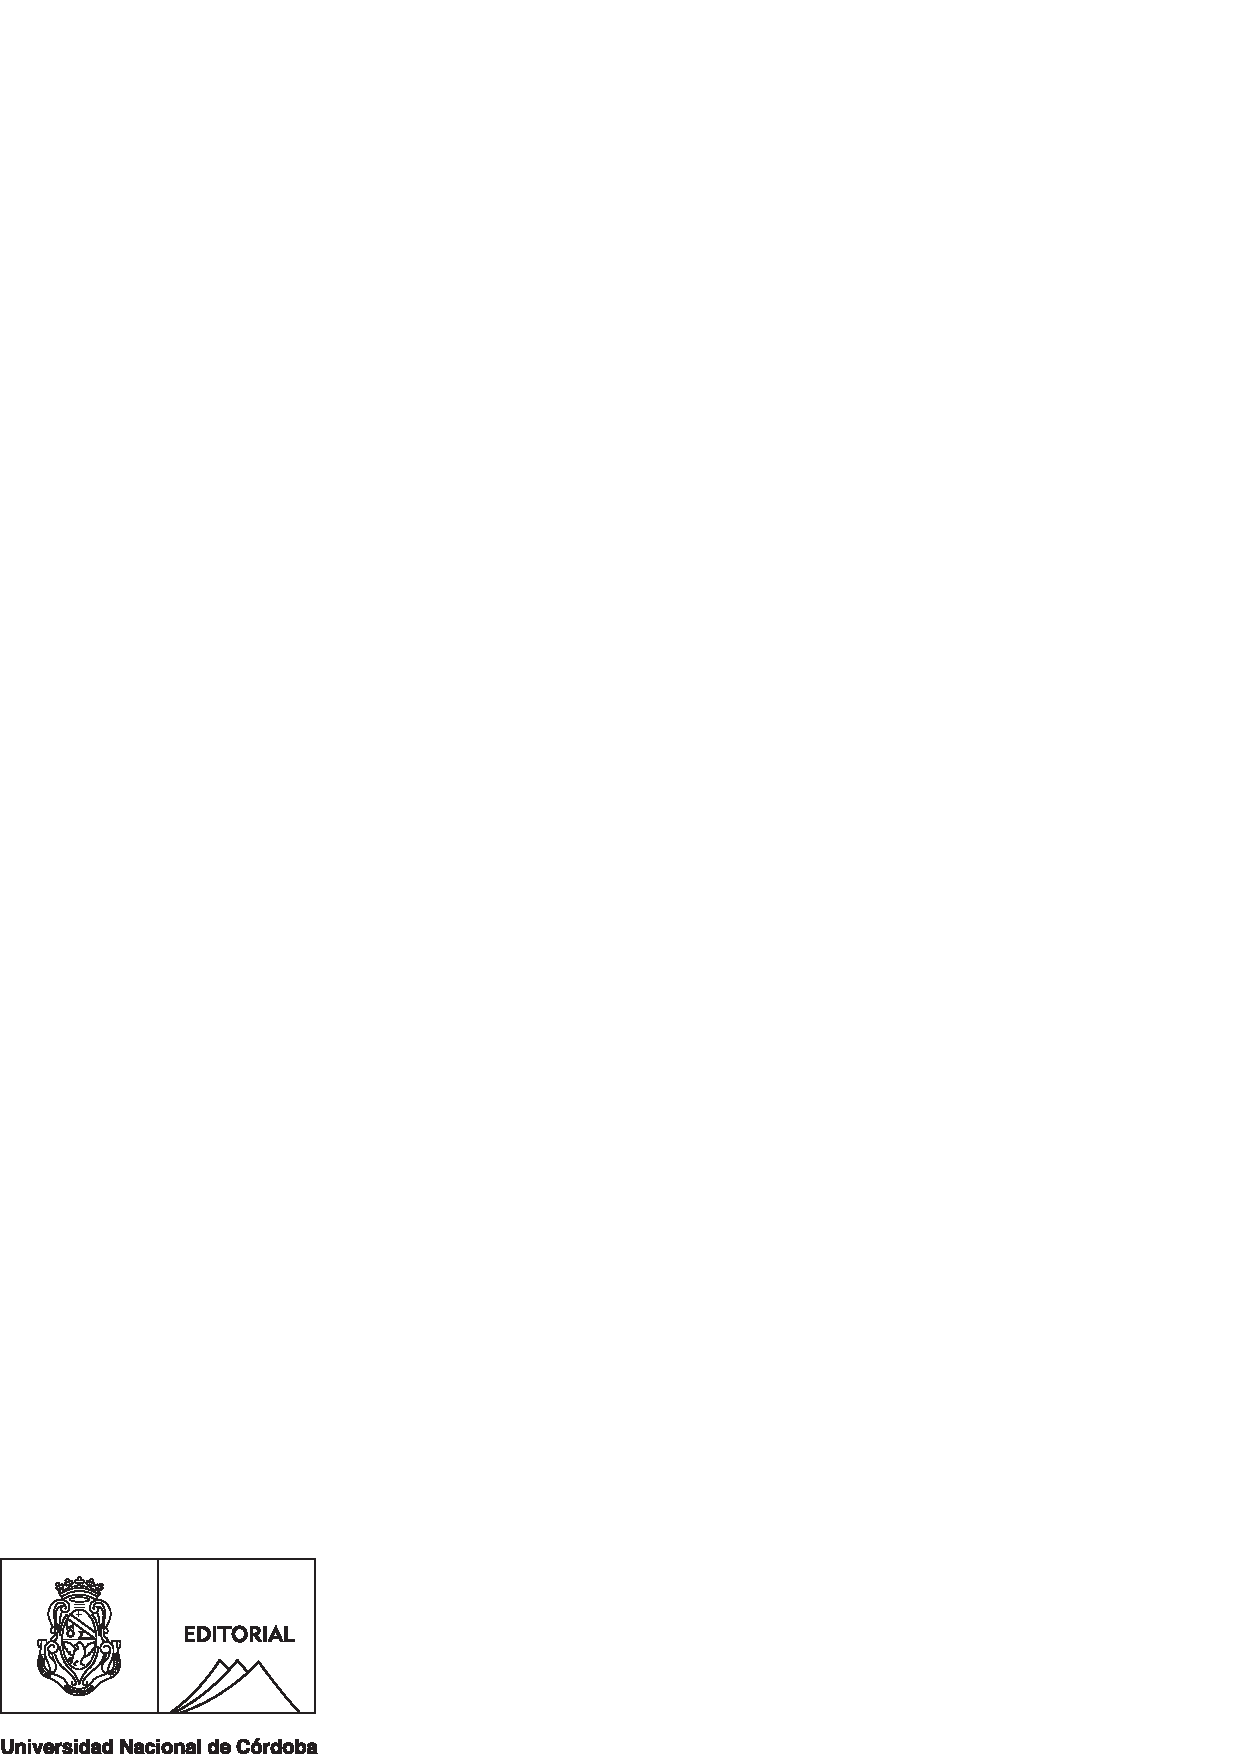
\includegraphics{Figure/logo.pdf}%
 \end{picture}
% }
    %\caption{Diagrama del operador dual.}
    %\label{fig:2_1}
%   \end{center}
% \end{figure}

%\maketitle
